% This is the file main.tex
\usepackage{group4}

\begin{document}
	
	\mode<article>{
		\newgeometry{margin=2in}
				\maketitle
				\restoregeometry
				\thispagestyle{empty}
				\newpage
				
				\textit{The following is just a collection of the discussions in preparation for turning what we have done into a write-up. This is not an actual write-up.}
		}
	
\begin{frame}
  \titlepage
\end{frame}

\titlepage

\mode<presentation>{
\section*{Outline}
\begin{frame}{Outline}
  \tableofcontents
\end{frame}
}

\mode<article>{
	\section{Achieving Stationarity}
	
	\subsection{Testing for Stationarity}
	\begin{itemize}
		\item I performed the ADF (augmented Dickey-Fuller) test for stationarity. We haven't talked about it in class yet, but it seems to be used pretty commonly. The high p-value suggests that we do not have a stationary model with just the raw unemployment data. This is confirmed with the non-constant variance and time-dependent mean that we observed in our exploratory analysis.
	\end{itemize}}
		
\begin{center}
	\textbf{Augmented Dickey-Fuller Test}
\end{center}
\begin{multicols}{2}

data:  unem \newline
Dickey-Fuller = -1.4266, Lag order = 6, \newline
p-value = 0.8176 \newline
alternative hypothesis: stationary 

data:  unem.sa \newline
Dickey-Fuller = -2.1377, Lag order = 6, \newline
p-value = 0.518 \newline
alternative hypothesis: stationary

\end{multicols}

	
	\subsection{Initial Plots}
	
			
\begin{figure}[H]
\centering
\caption{Plot of the original data}
\label{fig:unemployment}
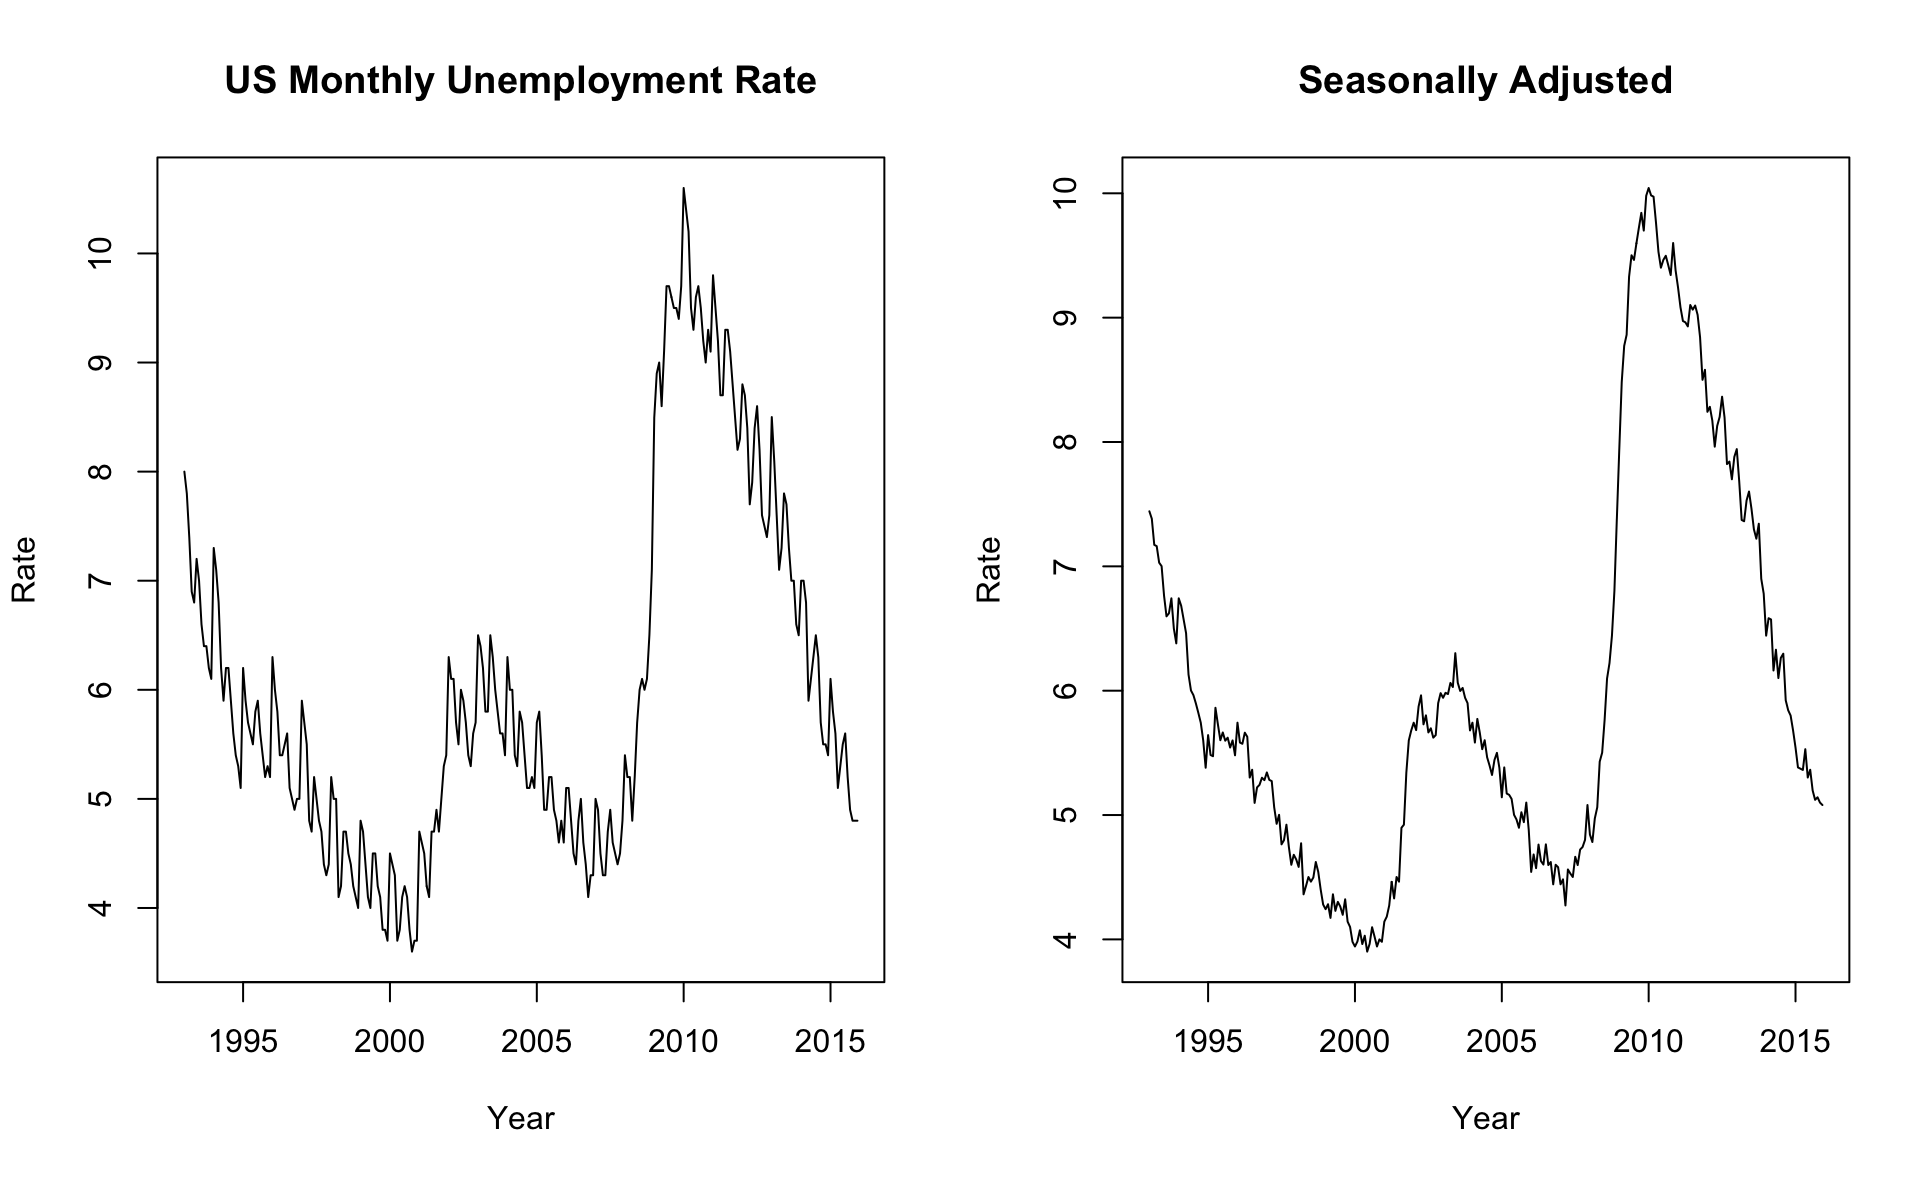
\includegraphics[width=\linewidth]{images/Unemployment}
\end{figure}

			
			\begin{multicols}{2}
						I then plotted the first difference, and it appears relatively stationary.
						
							This is confirmed by the ADF test on the first differenced data, which has a very small p-value:
						
						Augmented Dickey-Fuller Test
						Dickey-Fuller = -4.3501, Lag order = 6, p-value = 0.01
						alternative hypothesis: stationary
						
						\begin{figure}[H]
							\centering
							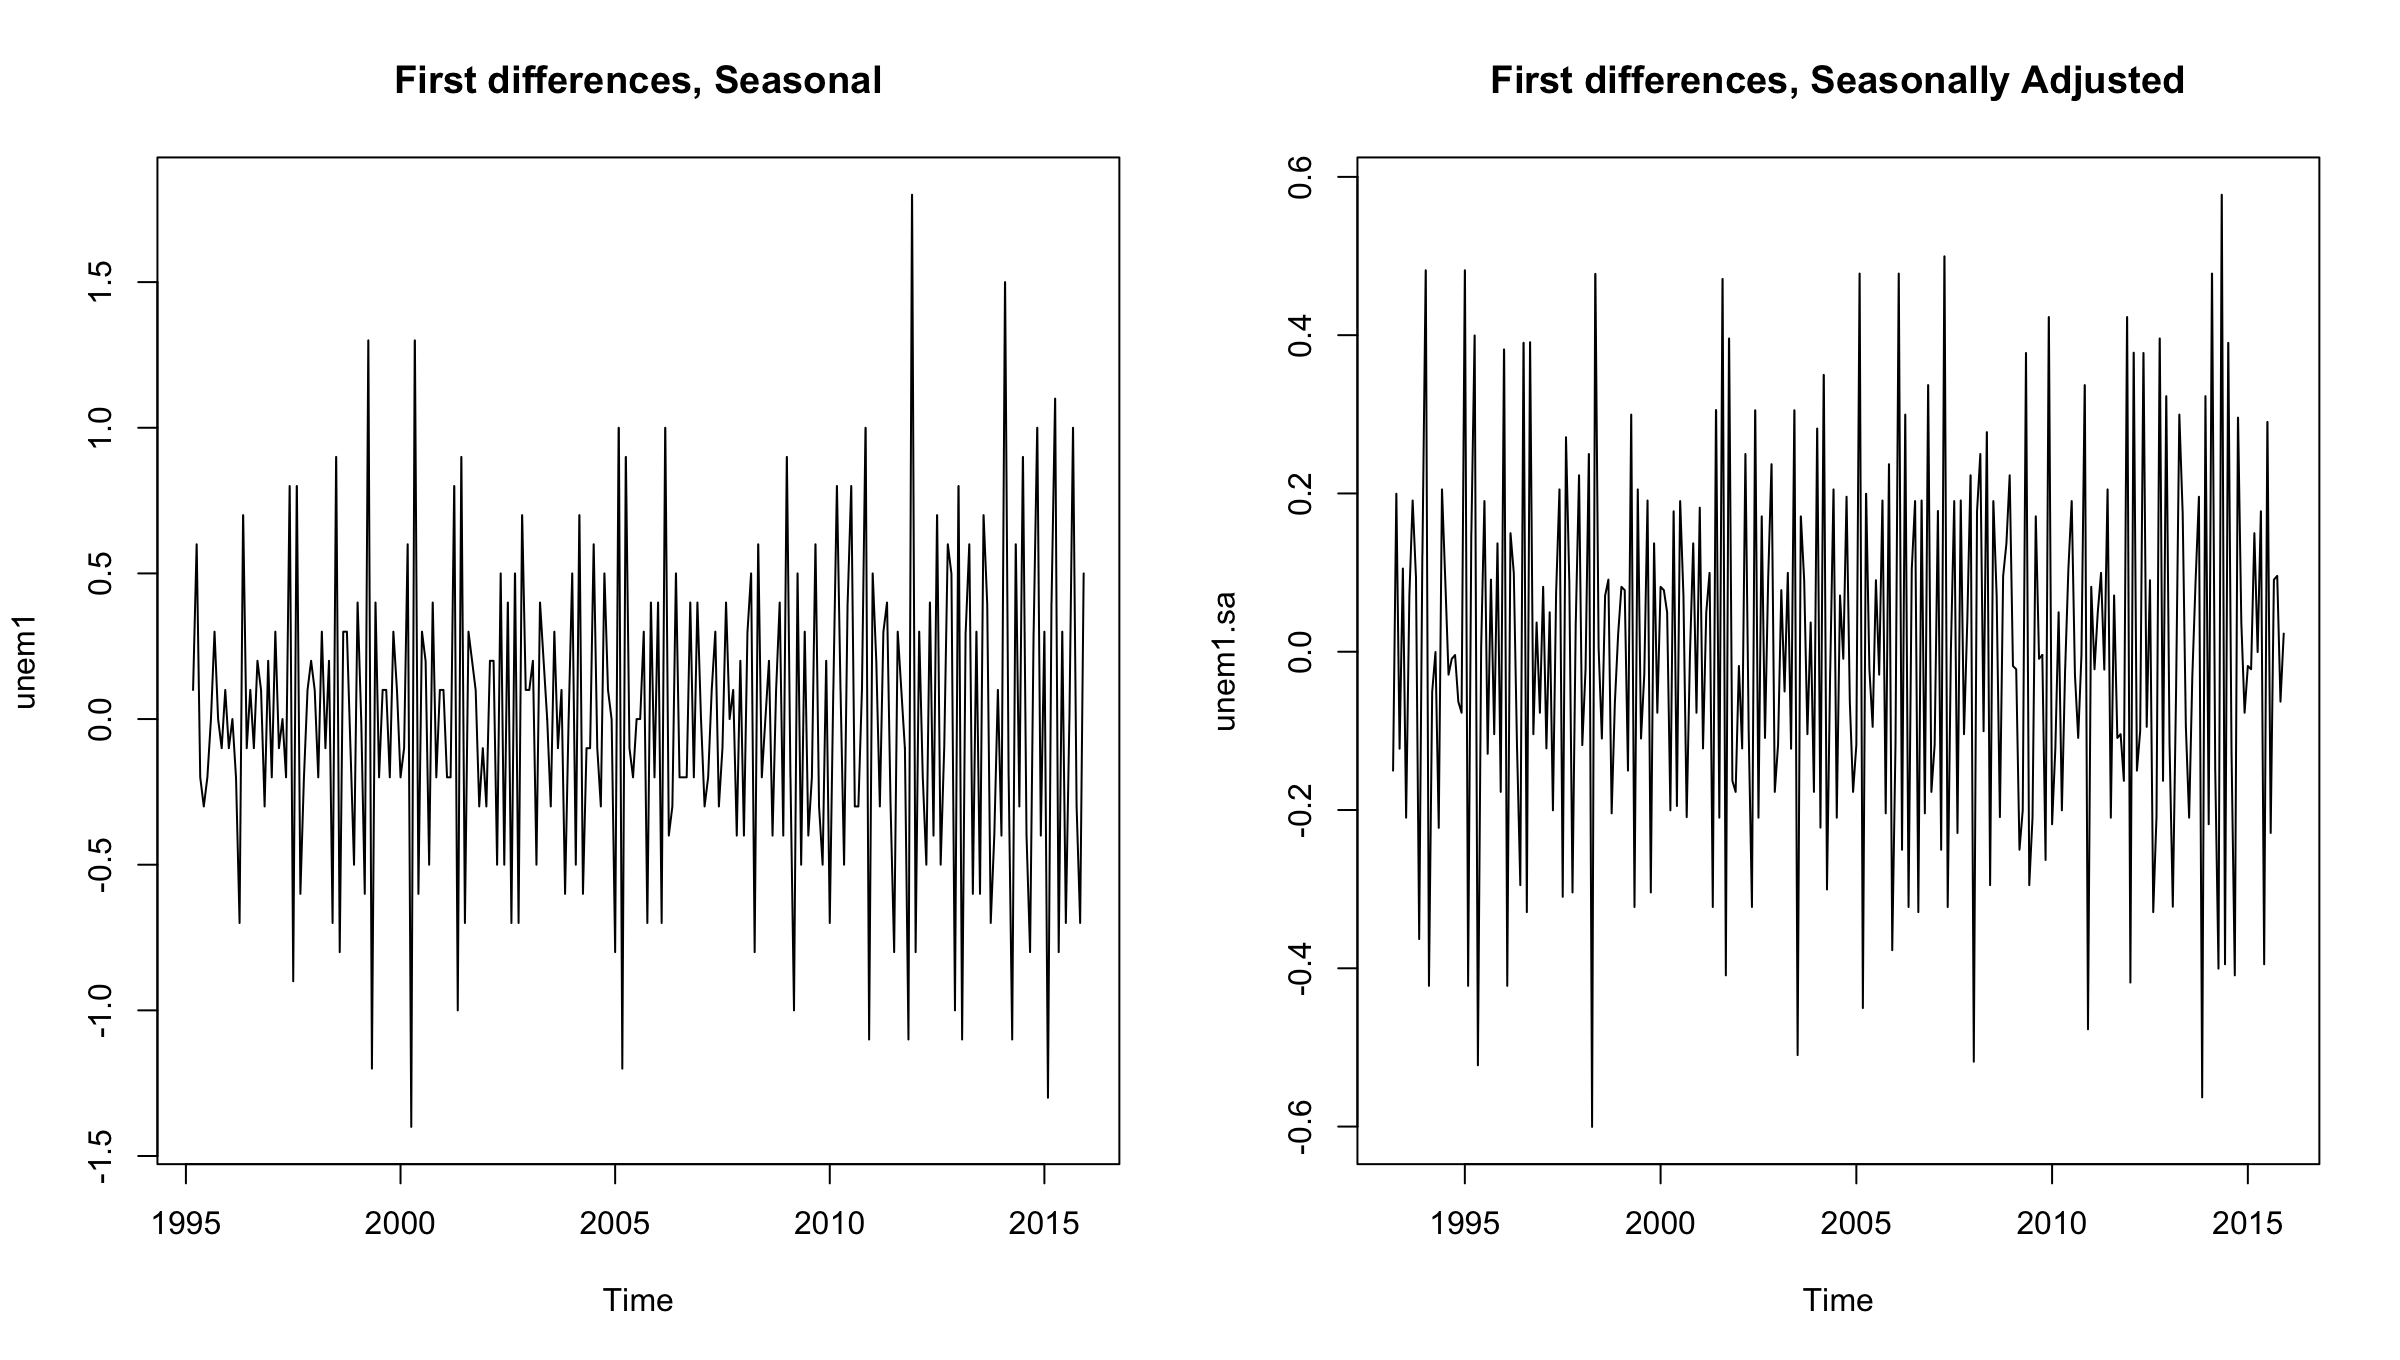
\includegraphics[width=.6\linewidth]{images/firstdiff}
							\caption{Plot of first Difference}
							\label{fig:firstdiff}
						\end{figure}
			\end{multicols}

	


\mode<presentation>{\section{Initial Plots}}

%-----------------------------------------------------------------------------------------
  \subsection{Differencing}
  
\begin{itemize}
	\item I took the second difference (d = 2), as Joseph suggested, then the first seasonal difference (D = 1) with s = 12 (this is common for monthly economic data), as the book did.
      
    \item   Below, Figure \ref{fig:secdiff},  is the plot of the transformed graphed. It looks pretty stationary (not perfect, but adequate), and we can confirm this with the ADF test (it's cited in other time series texts, but I haven't seen it in ours yet).
\end{itemize}
      
      \textit{I like the idea of using the ADF. We can include it as part of our literature review.}
      
      
      \begin{figure}[H]
      	\centering
      	\caption{Second differences with and without seasonal adjustments}
      	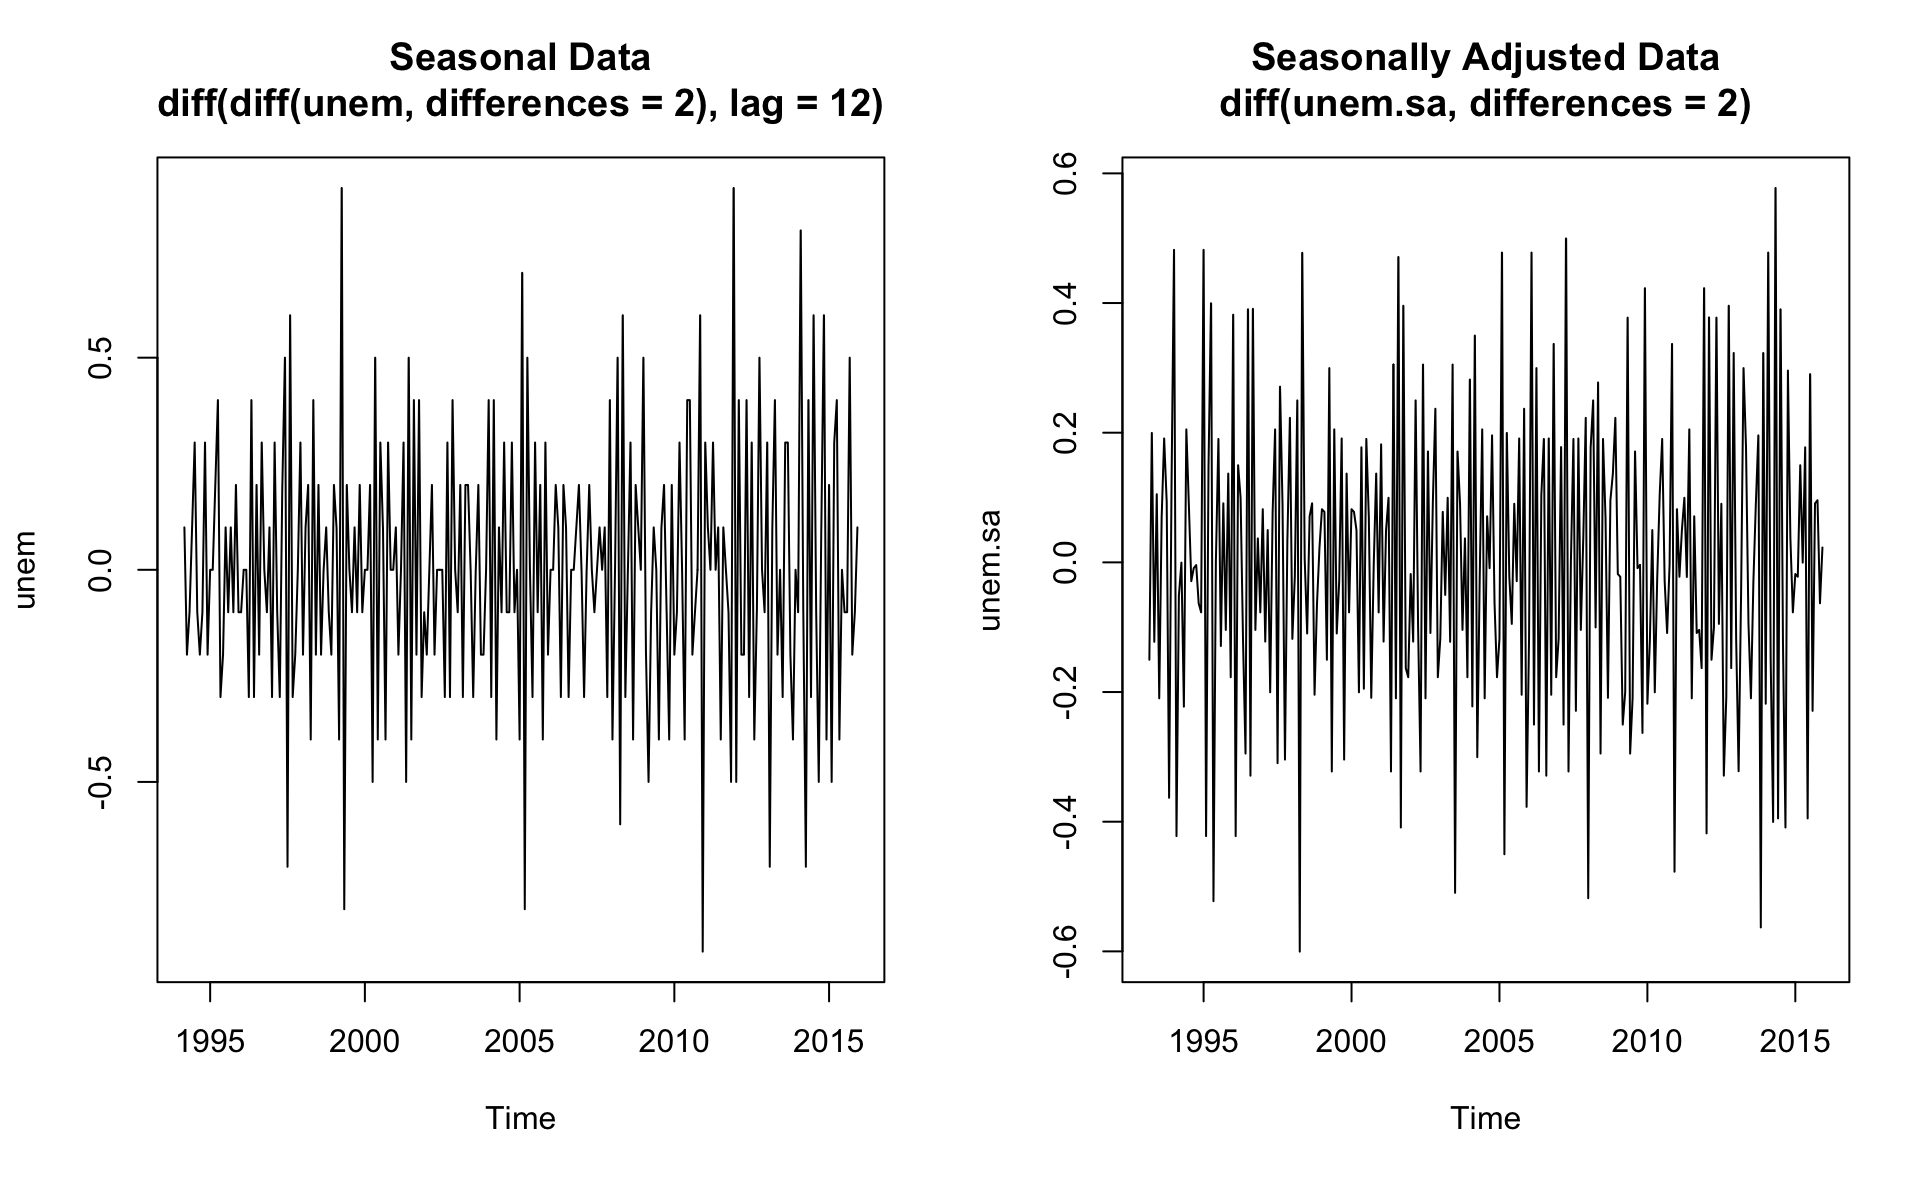
\includegraphics[width=.7\linewidth]{images/stationarity}
      	\label{fig:secdiff}
      \end{figure}
      

    

  
  \mode<presentation>{
  	\begin{frame}{Second differences with and without seasonal adjustments}
  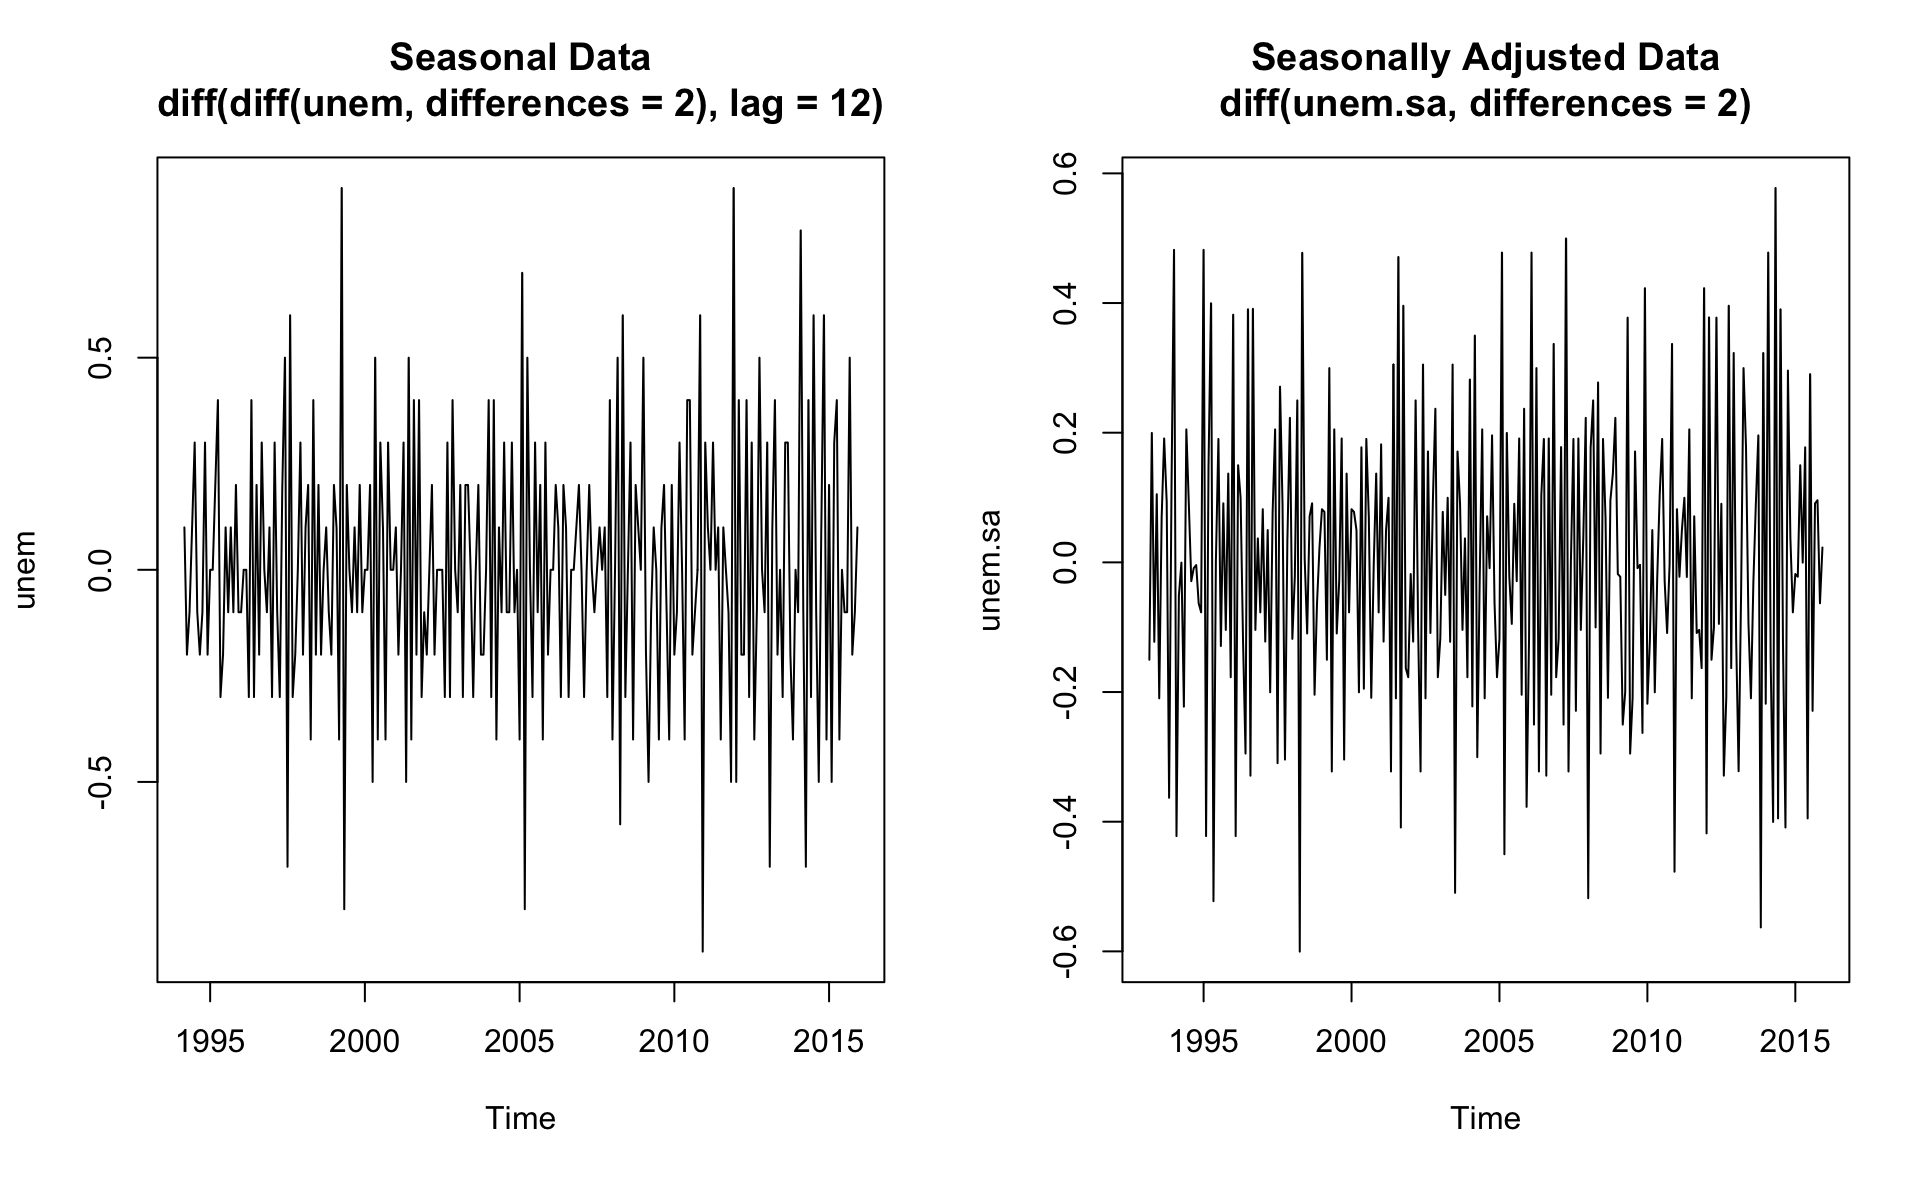
\includegraphics[width=.9\linewidth]{images/stationarity}
  \end{frame}
  }
  

%-----------------------------------------------------------------------------------------
  
  \subsection{ACF \& PACF}
  \begin{itemize}
  	\item  After that, the book suggests that you examine the ACF and PACF plots.
  	 \item First, the book says to look at the seasonal changes in ACF and PACF (h = 12, 24, 36, ...). These seem to indicate that the ACF trails off, and the PACF cuts off after one year (h = 12). This suggests that we let P = 1 and Q = 0.
  	 \item Next, the book says to look at the ACF and PACF within only the first season (h = 1, 2, ..., 12). The PACF declines slowly, but the ACF cuts off after 1, suggesting we let p = 0, and q = 1.
  \end{itemize}
  
   \mode<presentation>{
   	 \begin{frame}{ACF \& PACF Plots}
  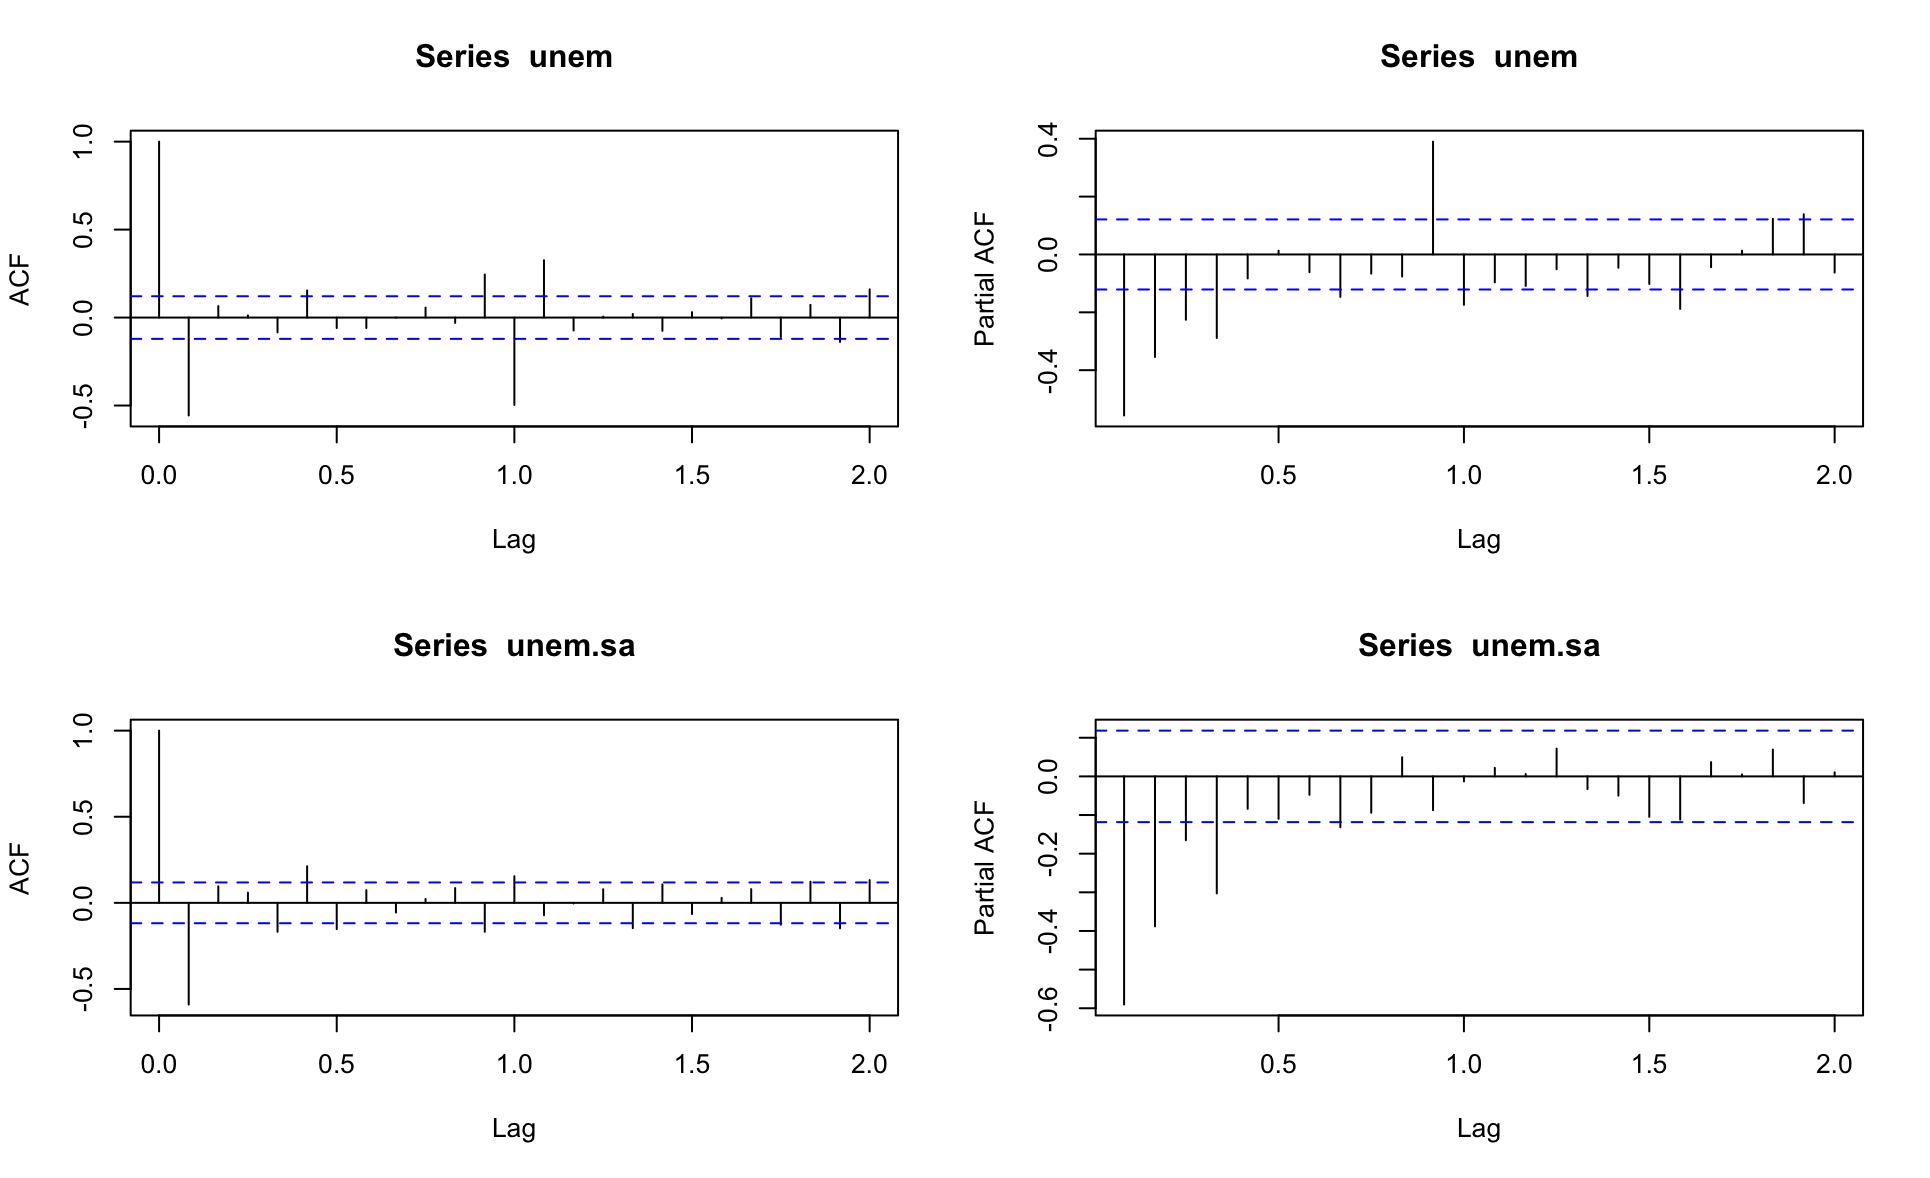
\includegraphics[width=.9\linewidth]{images/acfpacf}
  \end{frame}
}

      \begin{figure}[H]
      	\centering
      	\caption{ACF \& PACF Plots}
      	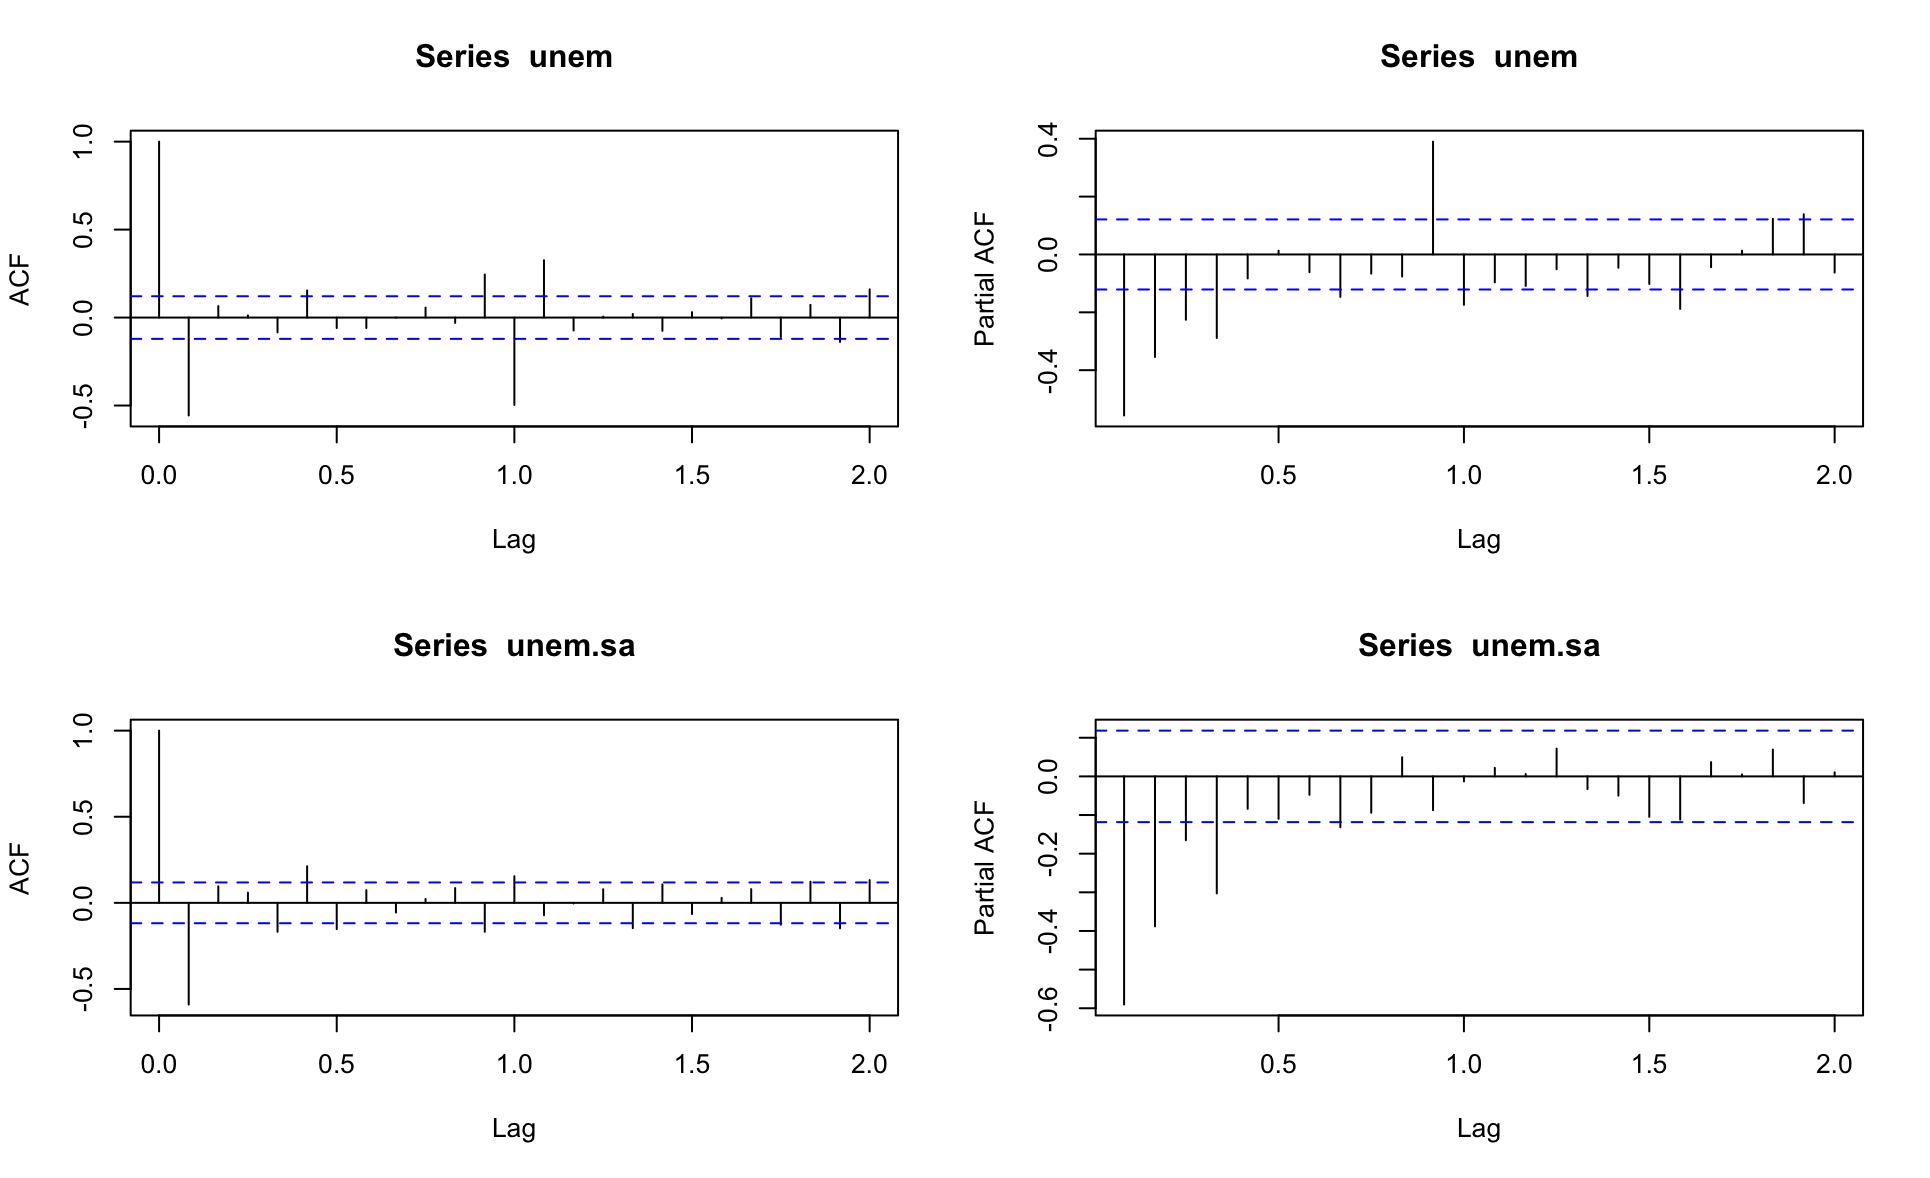
\includegraphics[width=\linewidth]{images/acfpacf}
      	\label{fig:secdiff2}
      \end{figure}
%----------------------------------------------------------------------------------------- 

    \section{Model Comparisons}
    
\begin{itemize}
	\item     I then look at the ACF and PACF plots to build models. First, we can look into the seasonal pattern. The ACF seems to tail off and the PACF cuts off at either 1 or 3. Together, the plots suggest AR(1) or AR (3).

\item We then can inspect the plots at the within season lags, h=1,..,11. One perspective is that the ACF cuts off after 1 and the PACF tails off, and it indicates MA(1). Another perspective is that the ACF cuts off after 1 and the PACF cuts off after 4. In this situation, the book suggests to build a SARMA of orders p = 4 and q = 1. However, our professor points out that this is a bad reasoning. It is still however tempting for me to try this model since I lean to the side that the PACF cuts off after lag 4 instead of tails off (some subjective feeling goes in here). We right now don't know how to handle the situation where both ACF and PACF cuts off at a certain lag other than the approach mentioned in the book. So I tried this model. In diagnostic procedures, as you will see, it works better at some criterion. Together, I proposed two additional models and compare them to the one proposed by Travis.

 \item  From looking at AIC and BIC values, Models 2 and 3 perform quite similarly, which both show some slight evidence of outperforming Model1.
  
  \item Then we could compare the three models based on diagnostic plots. The standardized residuals of all models show some evidence of non-white-noise. ARMA models do not model variability. We will have a few lectures on this topic. There is not much we can do now on this issue.
  
 \item  In the ACF of residuals of Model 1 shows a spike at lag 24. The other two models do not show such a spike.
  
  \item The normal plots from the three models are fairly similar.
  
  \item The Q-statistic or Ljung-Box statistic:
  
  Models 1 and 2 have similar results. Model 1 seems to perform better at the first few lags, but Model 2 does better after lag 15. Model 3 clearly perform better than the two models on the Q-statistic. Since the Model 3 is based on a reasoning our professor does not like, we may not present this model. However it at least informs us that some models based on the thought that both the ACF and PACF cuts off at certain lags might model our data better. 
  
 \item  While going through a bunch of models, the following model seems most appropriate as noted by everyone. sarima(econ[,2],0,2,1,1,1,0,12) with the following diagnostics: [image: Inline image 2] The adf test also suggests stationarity as follows:  Also, I am working on other predictor variables to develop a preliminary regression model.
  
 \item  I am trying to fit the regression model here and was wondering if I should
take the stationary data for my fitting? Any help on this would be
appreciated.

\item I believe you would need to use the stationary non-seasonal unemployment rate as your response variable. I do not believe your predictor variables have to be stationary, but it would probably make sense to at least take the seasonality out of them.

\item Checking both residual plots shows that there is a drastic drop that is likely indicative of the 2008 recession. Can we add weighting or something to fix this?

\item In the political dataset I have an indicator variable for recession by month we could try using that. 

\item Regarding the expectations for presentation, the professor has not mentioned yet. However, in the last two lectures (14 and 15), he talked a lot applied examples about model building. I'd assume that our presentation would be something similar to what he talked in the two lectures. Basically, it's the model building process. How do we preprocess our data to obtain a stationary process (difference order 2 and difference order 1 in our case)? How do we identify the model (based on ACF and PACF)? What is the set of candidate models? How do you choose the best one (AIC, BIC, diagnostics)? I guess we might not need to present a regression model at this stage since he hasn't talked much about it. How do you guys think about this?

\item "Best model," as far as I know, is pretty ambiguous right now. With what I have done before, I checked AIC and BIC (not really thinking about using R-squared for the time being). The model identification from P/ACF is outlined in the text by checking out the tail behavior to see if it decays asymptotically or cuts off. We should be checking inside the band for "cutoff" behavior.

\item Sure, it's always hard to call a model "Best". I think in presentations, we may present several potential candidate models, and compare them from several perspectives. Hopefully, one model will gain relatively more evidence.

\item I would like to propose an additional model. I have gone through the same exercise as @trlilley12 and @bopangpsy only I used the seasonally adjusted unemployment rate. It looks like the performance is definitely comparable to the seasonal models. I used sarima for the nice diagnostic plot it creates, but I left the seasonal parameters out.

\end{itemize}

I get an AICc \(= -2.617631\) and BIC \(= -3.598962\)

\begin{verbatim}
mdl4 = sarima(xdata = unem, p = 1, d = 2, q = 1)

Call:
stats::arima(x = xdata, order = c(p, d, q), seasonal = list(order = c(P, D, 
Q), period = S), include.mean = !no.constant, optim.control = list(trace = trc, 
REPORT = 1, reltol = tol))

Coefficients:
ar1      ma1
-0.2021  -0.8078
s.e.   0.0688   0.0433

sigma^2 estimated as 0.02626:  log likelihood = 109.15,  aic = -212.3

$AIC
[1] -2.625197

$AICc
[1] -2.617631

$BIC
[1] -3.598962
\end{verbatim}

Cool, Joseph! This model is simple and performs pretty well in terms of both fitting indices and diagnostics.
    
%-----------------------------------------------------------------------------------------    
    \subsection{Overview}
  \begin{frame}{Models Considered}
    % latex table generated in R 3.2.4 by xtable 1.8-2 package
% Thu Jul  7 16:13:24 2016
\begin{table}[H]
\centering
\caption{Model Summaries}
\begin{tabular}{llccccc}
  \hline
 \textbf{\#}& \textbf{Data}  & \textbf{Order} & \textbf{Seasonal} & \textbf{XRegs} & \textbf{AIC} & \textbf{BIC} \\
 &&&\textbf{Order}&&&\\ 
  \hline
1 & Unem  & 0,2,1 & 1,1,0 & N & -2.27 & -3.23 \\ 
  2 & Unem  & 0,2,1 & 3,1,0 & N & -2.44 & -3.37 \\ 
  3 & Unem  & 4,2,1 & 3,1,0 & N & -2.44 & -3.32 \\ 
  4 & Unem.sa & 0,2,1 & 1,0,0 & N & -2.61 & -3.58 \\ 
  5 & Unem.sa  & 1,2,1 &  & N & -2.63 & -3.60 \\ 
  6 & Unem.sa & 0,2,1 & 1,0,0 & Y & -2.58 & -3.49 \\ 
  7 & Unem.sa  & 1,2,1 &  & Y & -2.60 & -3.49 \\ 
   \hline
\end{tabular}
\label{tab:models}
\end{table}
  \end{frame}
%-----------------------------------------------------------------------------------------

 \subsection{Seasonal Models}
 %-----------------------------------------------------------------------------------------
  \begin{frame}{Model 1: SARIMA\((0,2,1) \times (1,1,0)_{12}\)}
  		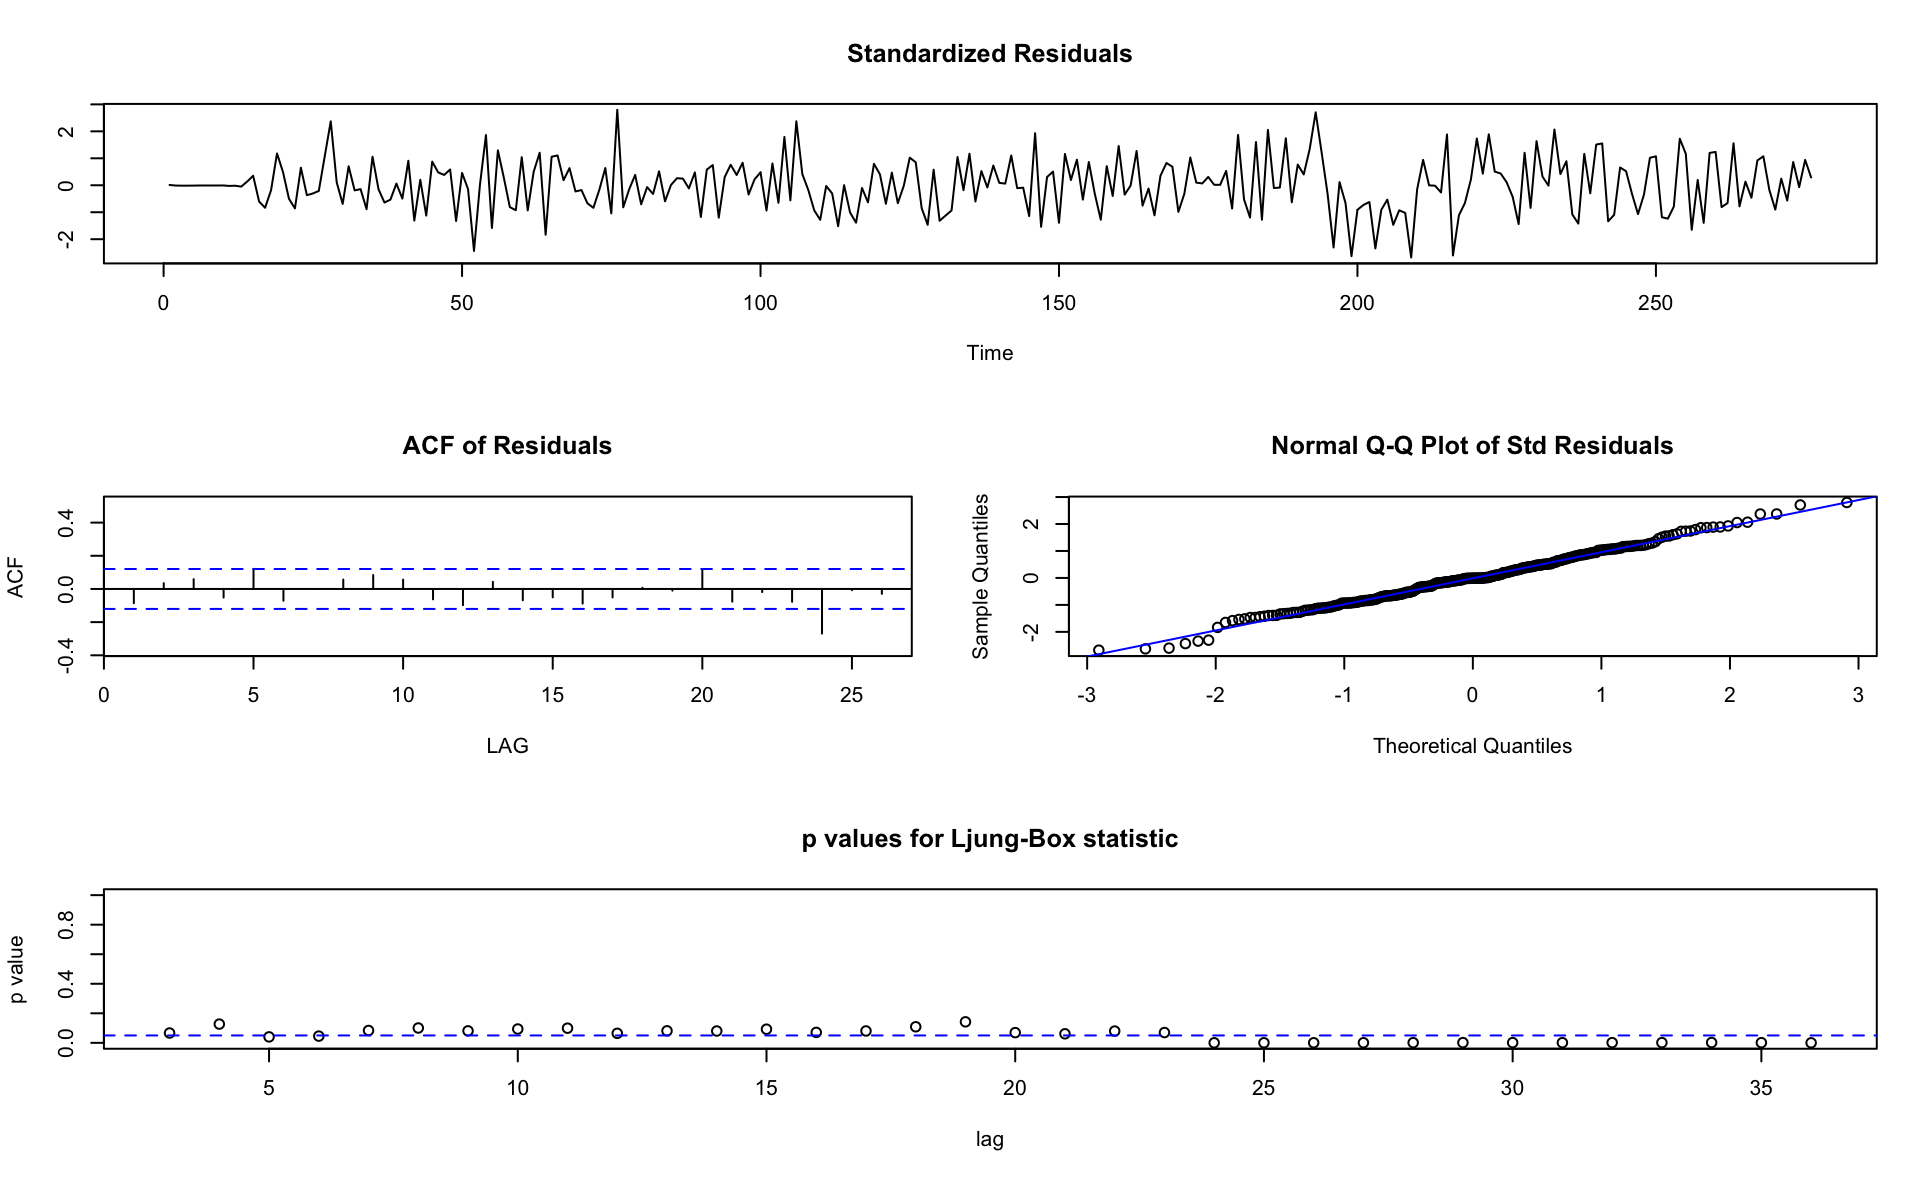
\includegraphics[width=\linewidth]{images/seasonalmodel1}
  \end{frame}

%-----------------------------------------------------------------------------------------

\begin{frame}{Model 2: SARIMA\((0,2,1) \times (3,1,0)_{12}\)}
  		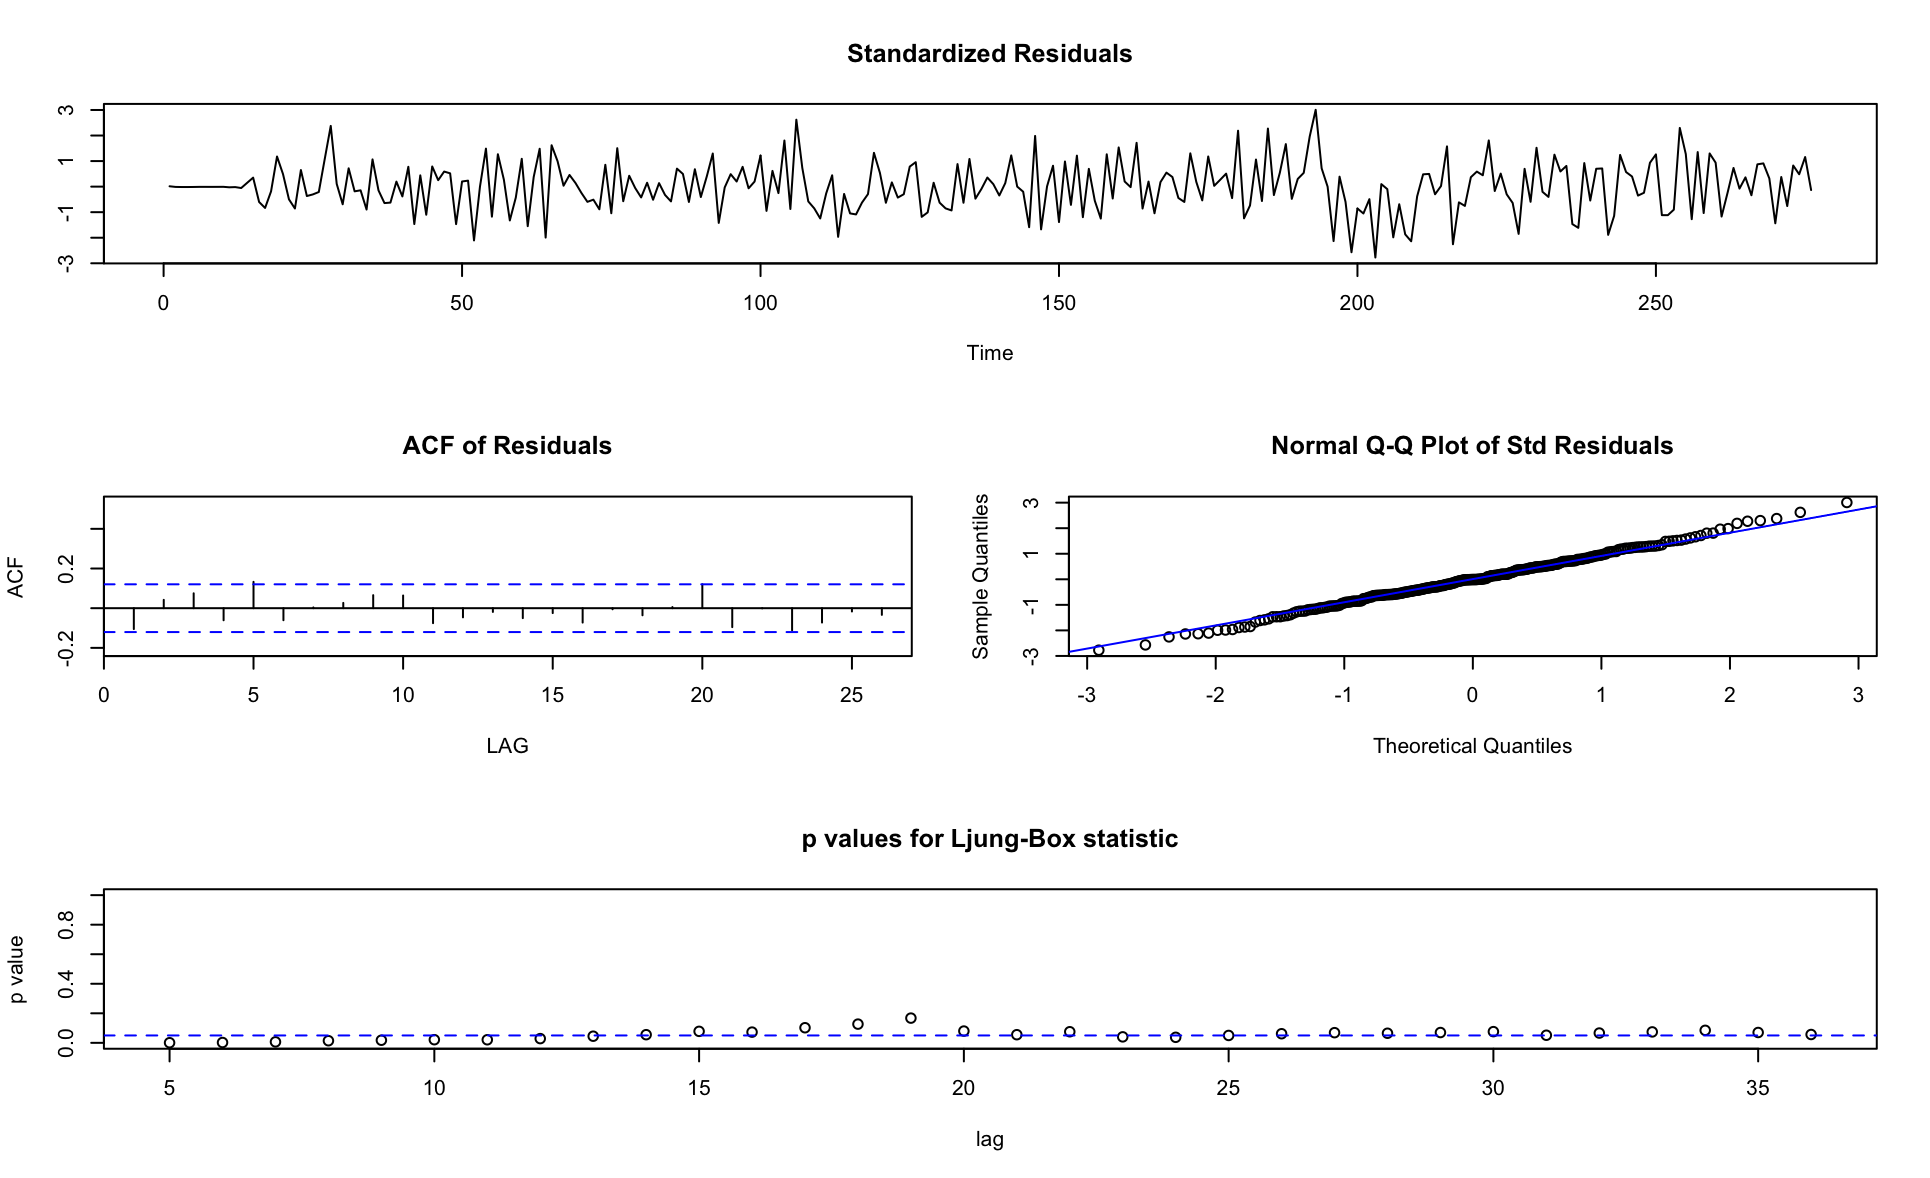
\includegraphics[width=\linewidth]{images/seasonalmodel2}
  \end{frame}  

%-----------------------------------------------------------------------------------------
  
  \begin{frame}{Model 3: SARIMA\((4, 2, 1) \times (3,1,0)_{12}\)}
  		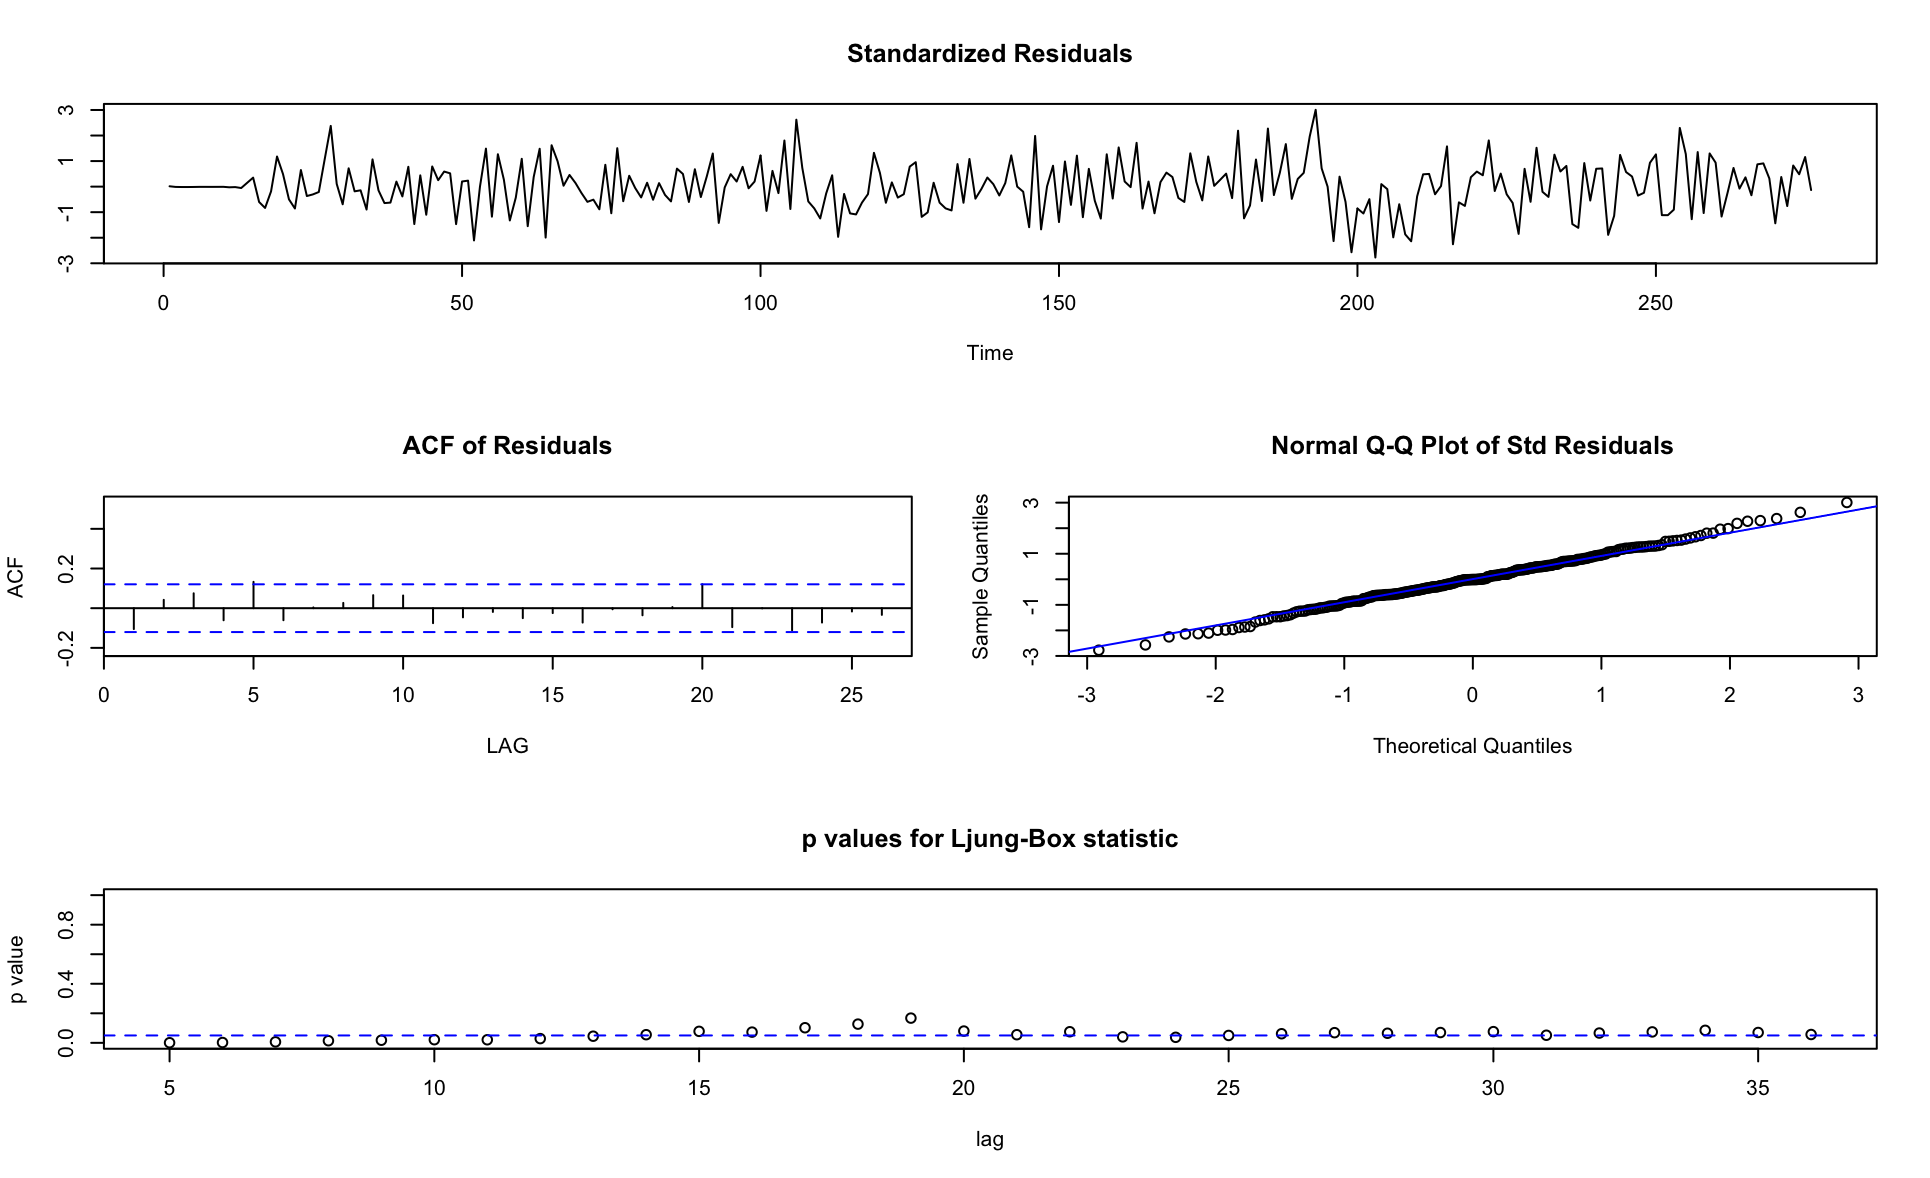
\includegraphics[width=\linewidth]{images/seasonalmodel3}
  \end{frame}  
%-----------------------------------------------------------------------------------------  

  \subsection{Seasonally Adjusted Models}
%-----------------------------------------------------------------------------------------  
  \begin{frame}{Model 4: SARIMA\((0,2,1) \times (1,0,0)_{12}\)}
  	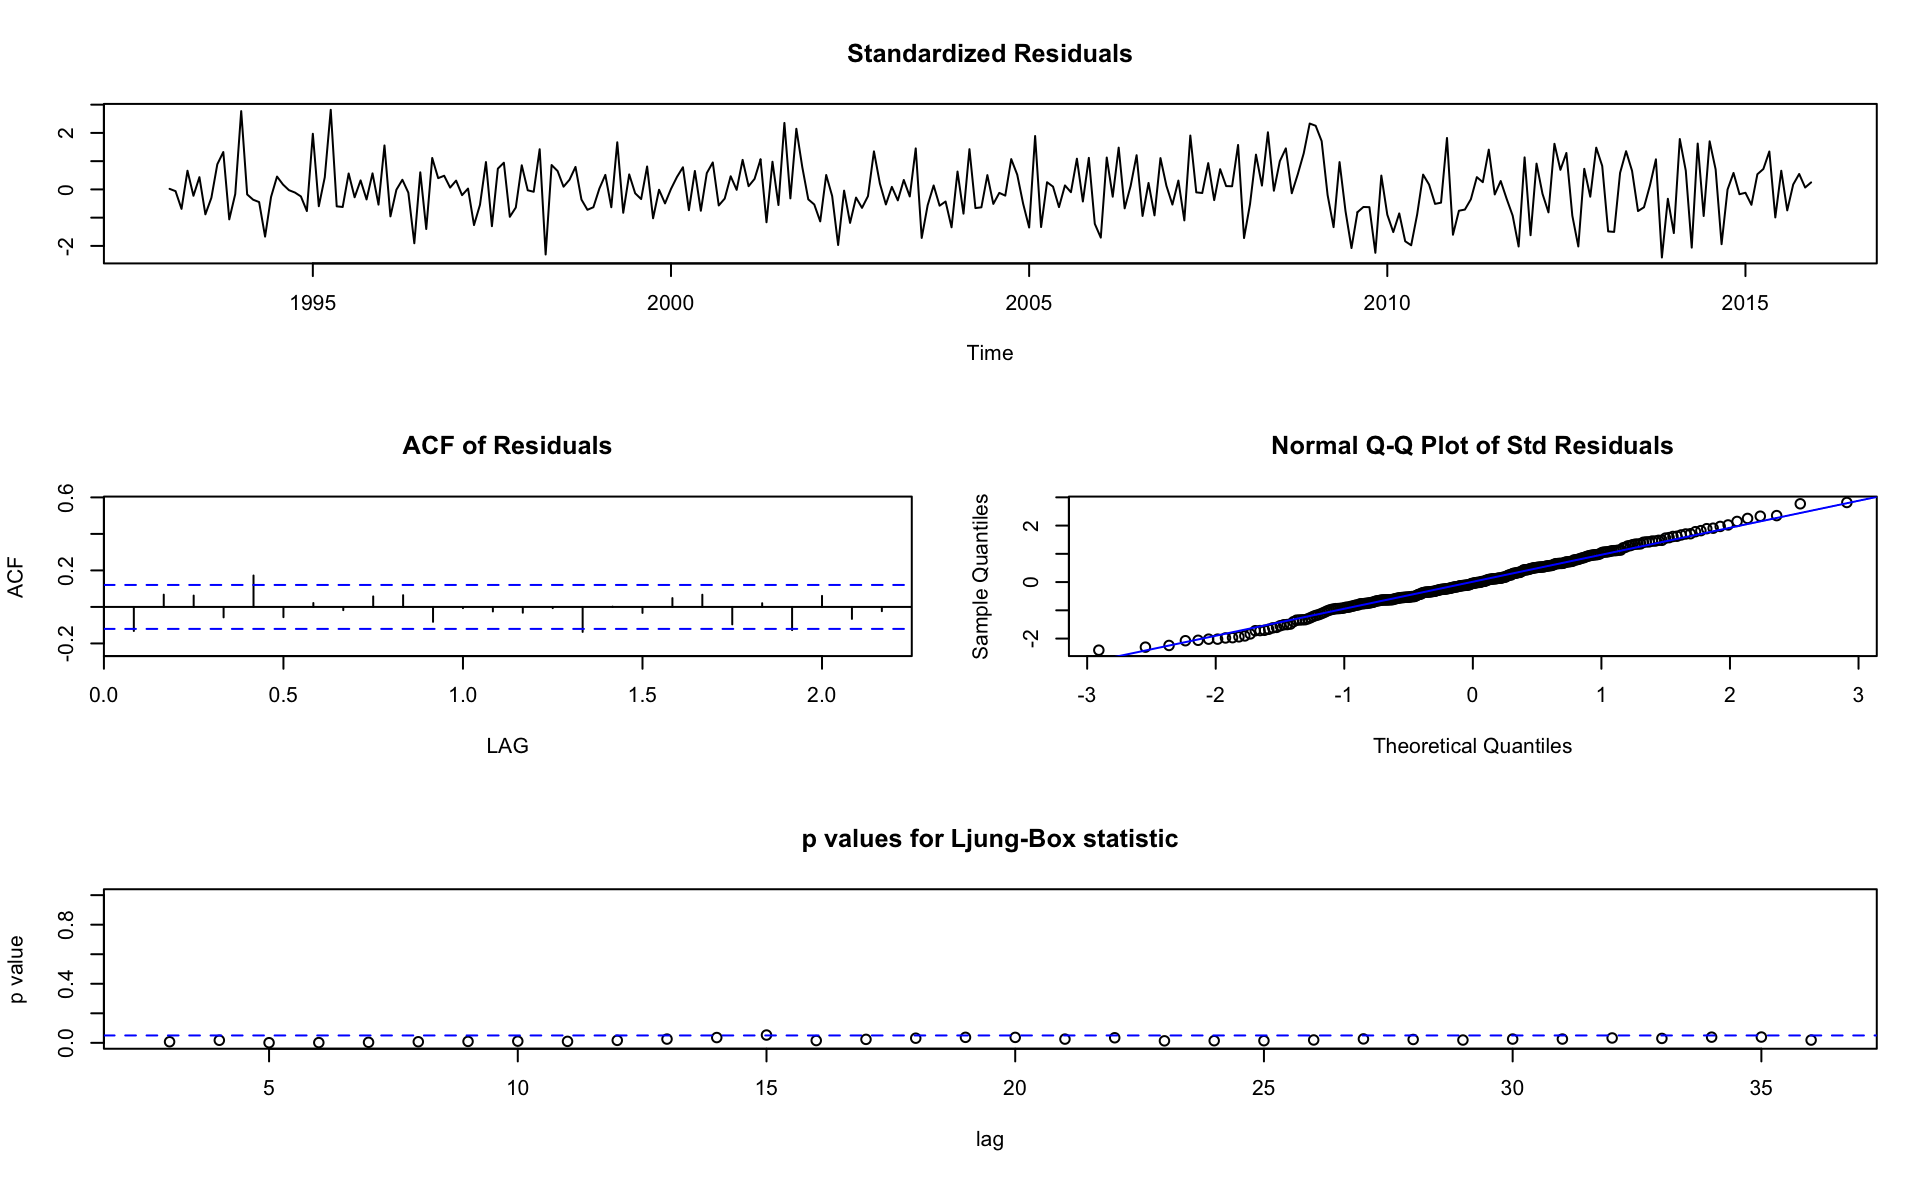
\includegraphics[width=\linewidth]{images/seasonallyadjustedmodel4}
  \end{frame}
  
%-----------------------------------------------------------------------------------------
  
  \begin{frame}{Model 5: ARIMA\((1,2,1)\)}
  		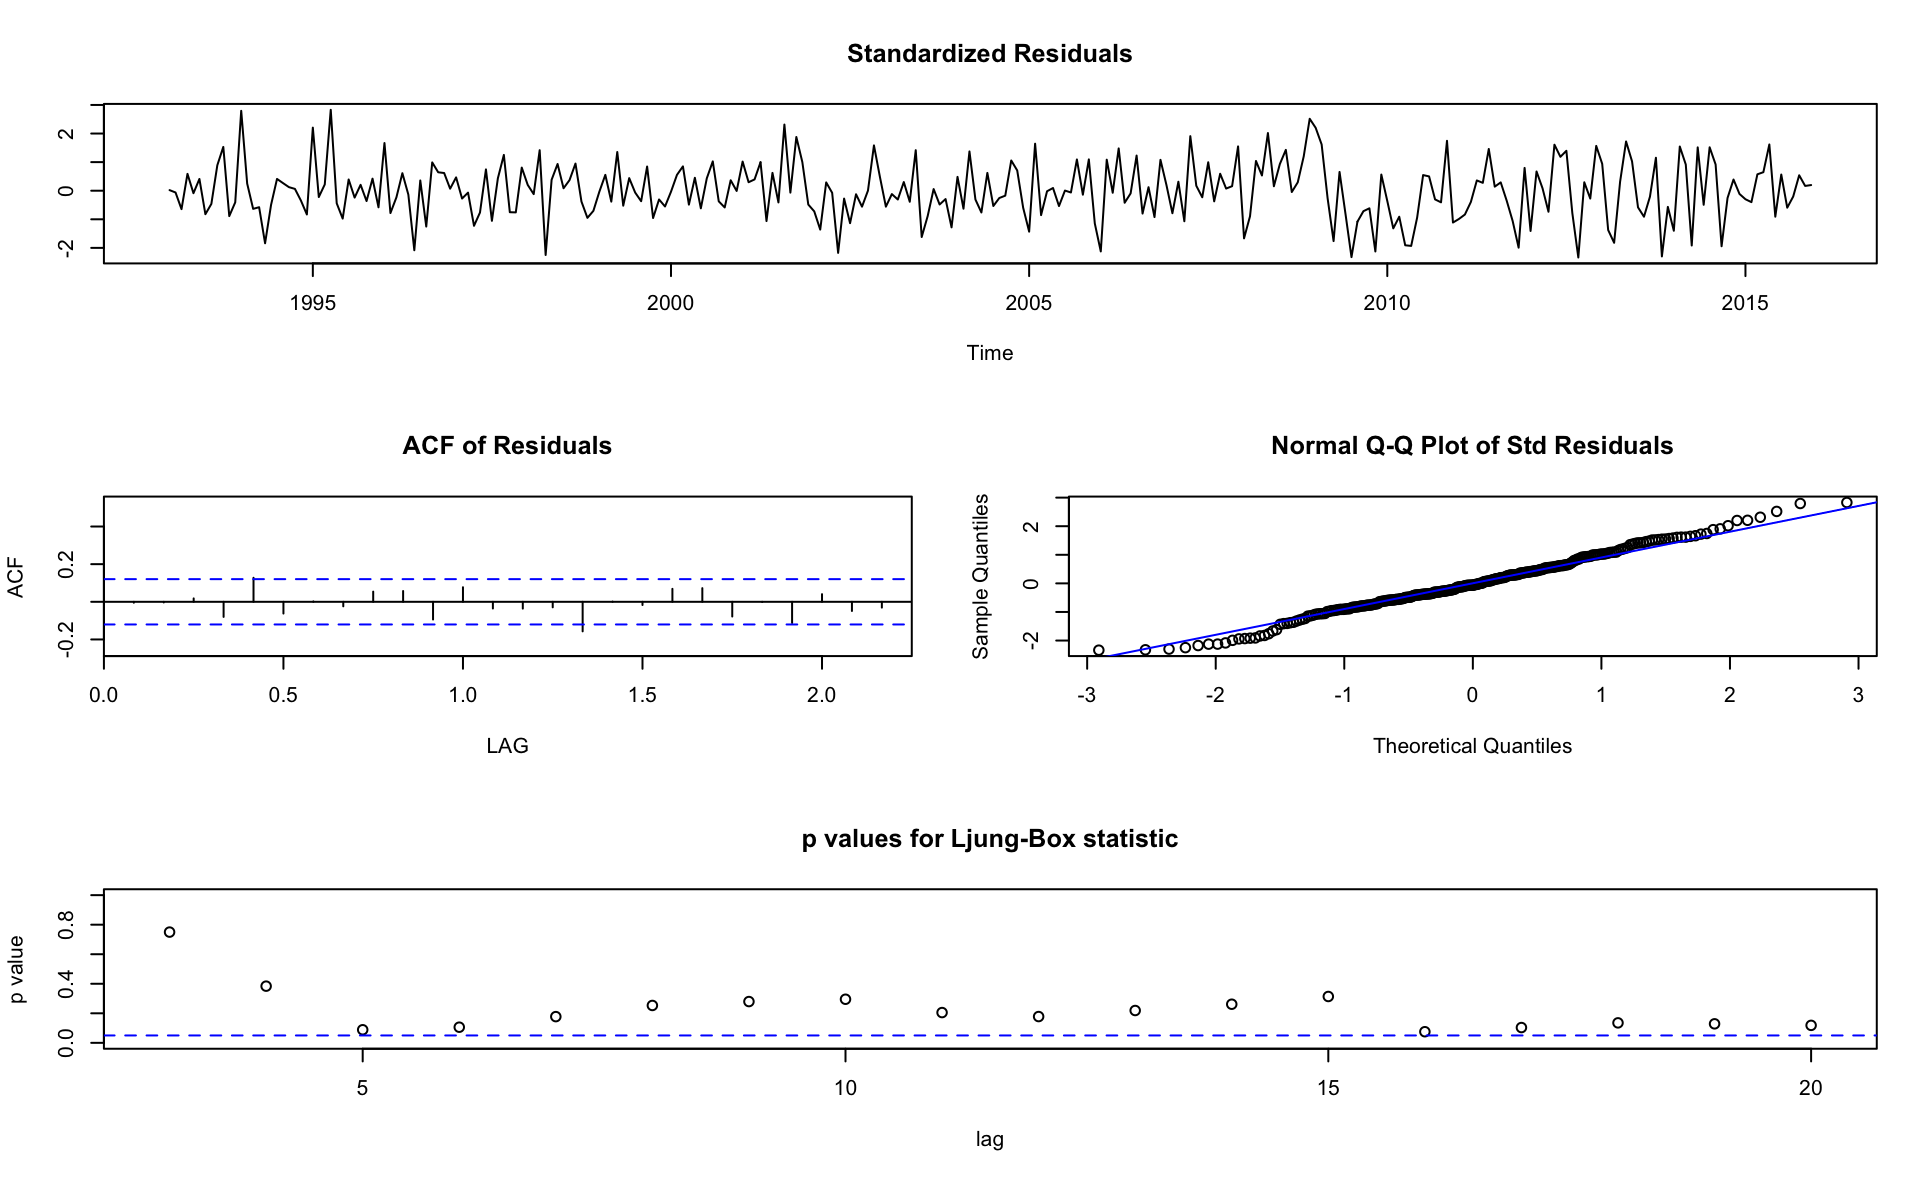
\includegraphics[width=\linewidth]{images/seasonallyadjustedmodel5}
  \end{frame}
  
  %-----------------------------------------------------------------------------------------
  
  \begin{frame}{Model 6: SARIMA\((0,2,1) \times (1,0,0)_{12}\) with Regressors}
  		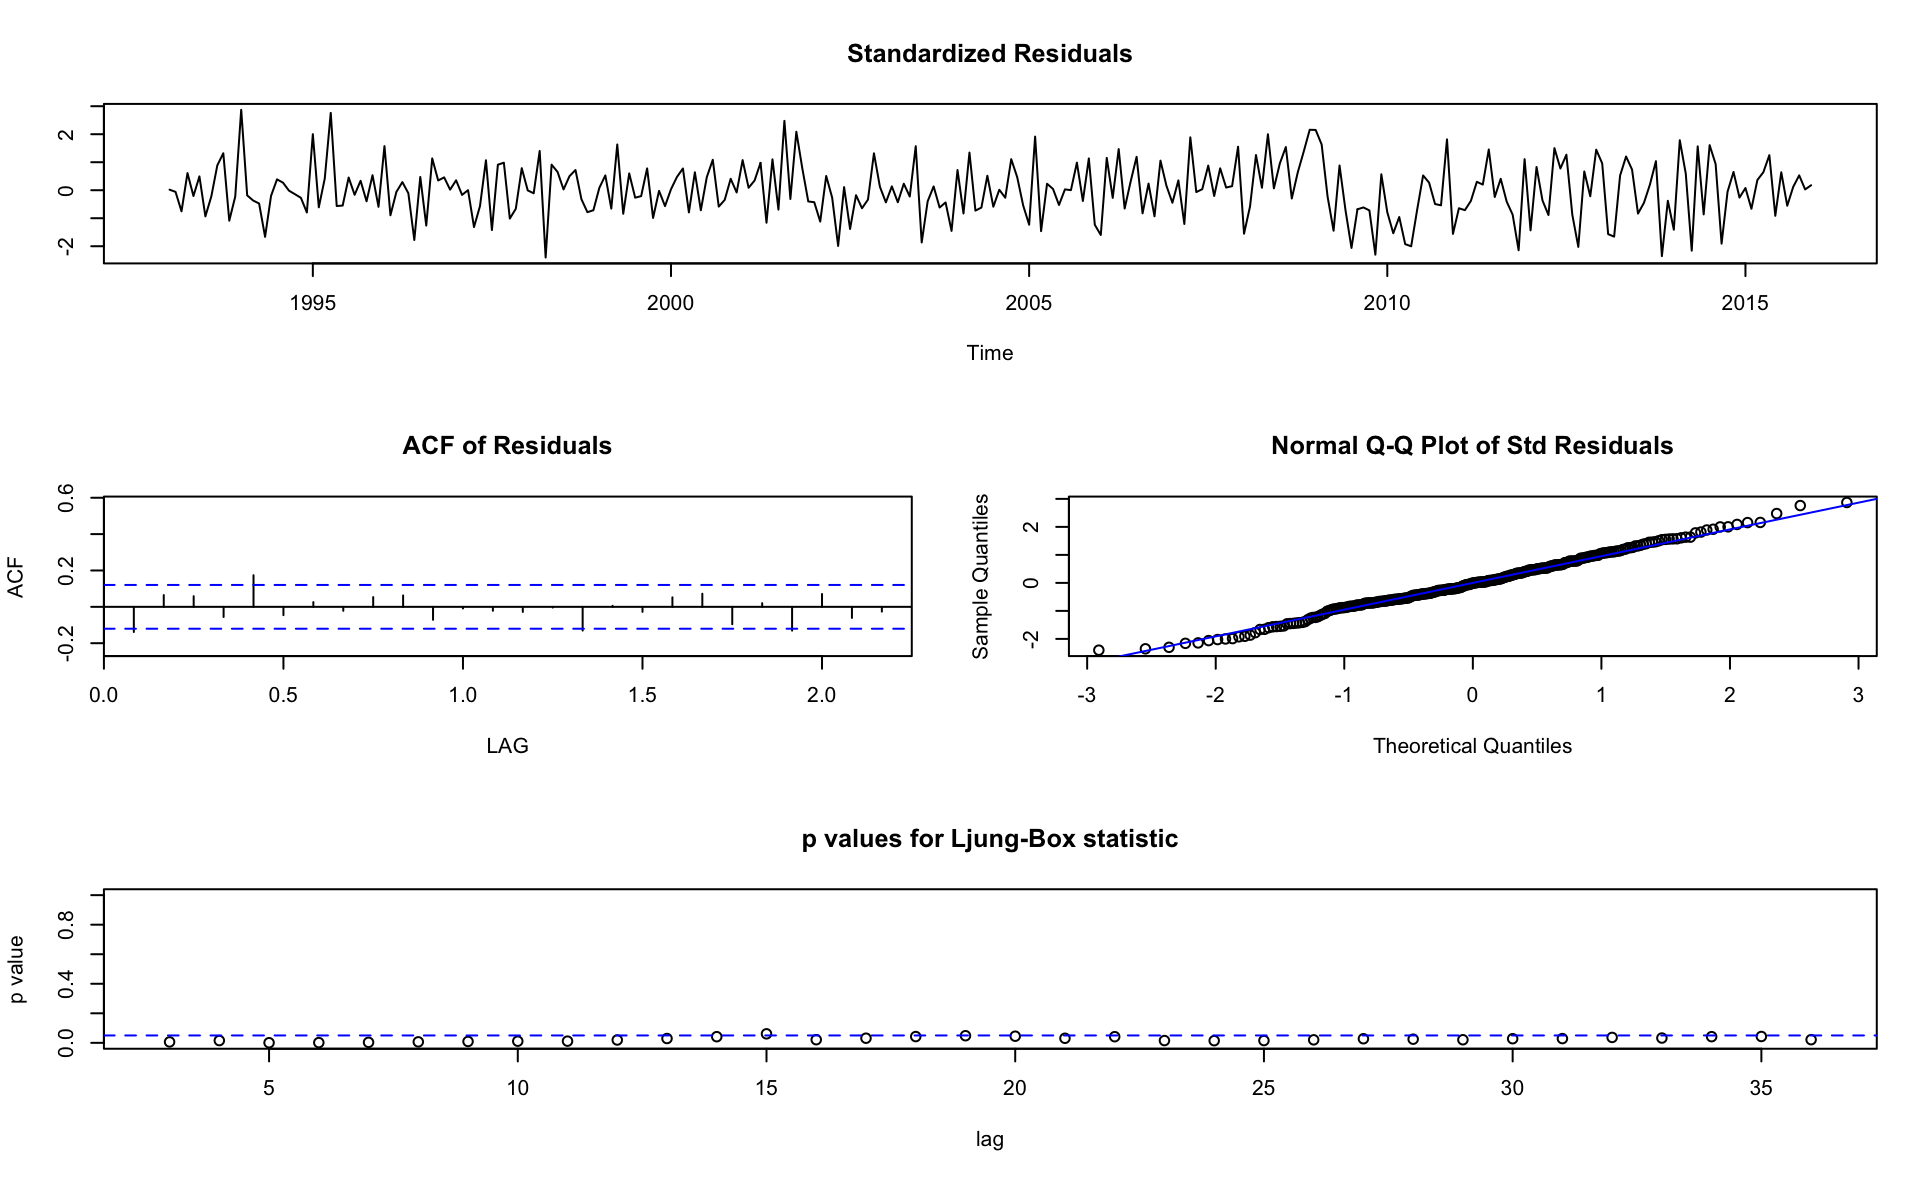
\includegraphics[width=\linewidth]{images/seasonallyadjustedmodel6}
  \end{frame}
  
  %-----------------------------------------------------------------------------------------
  
  \begin{frame}{Model 7: ARIMA\((1,2,1)\) with Regressors}
  		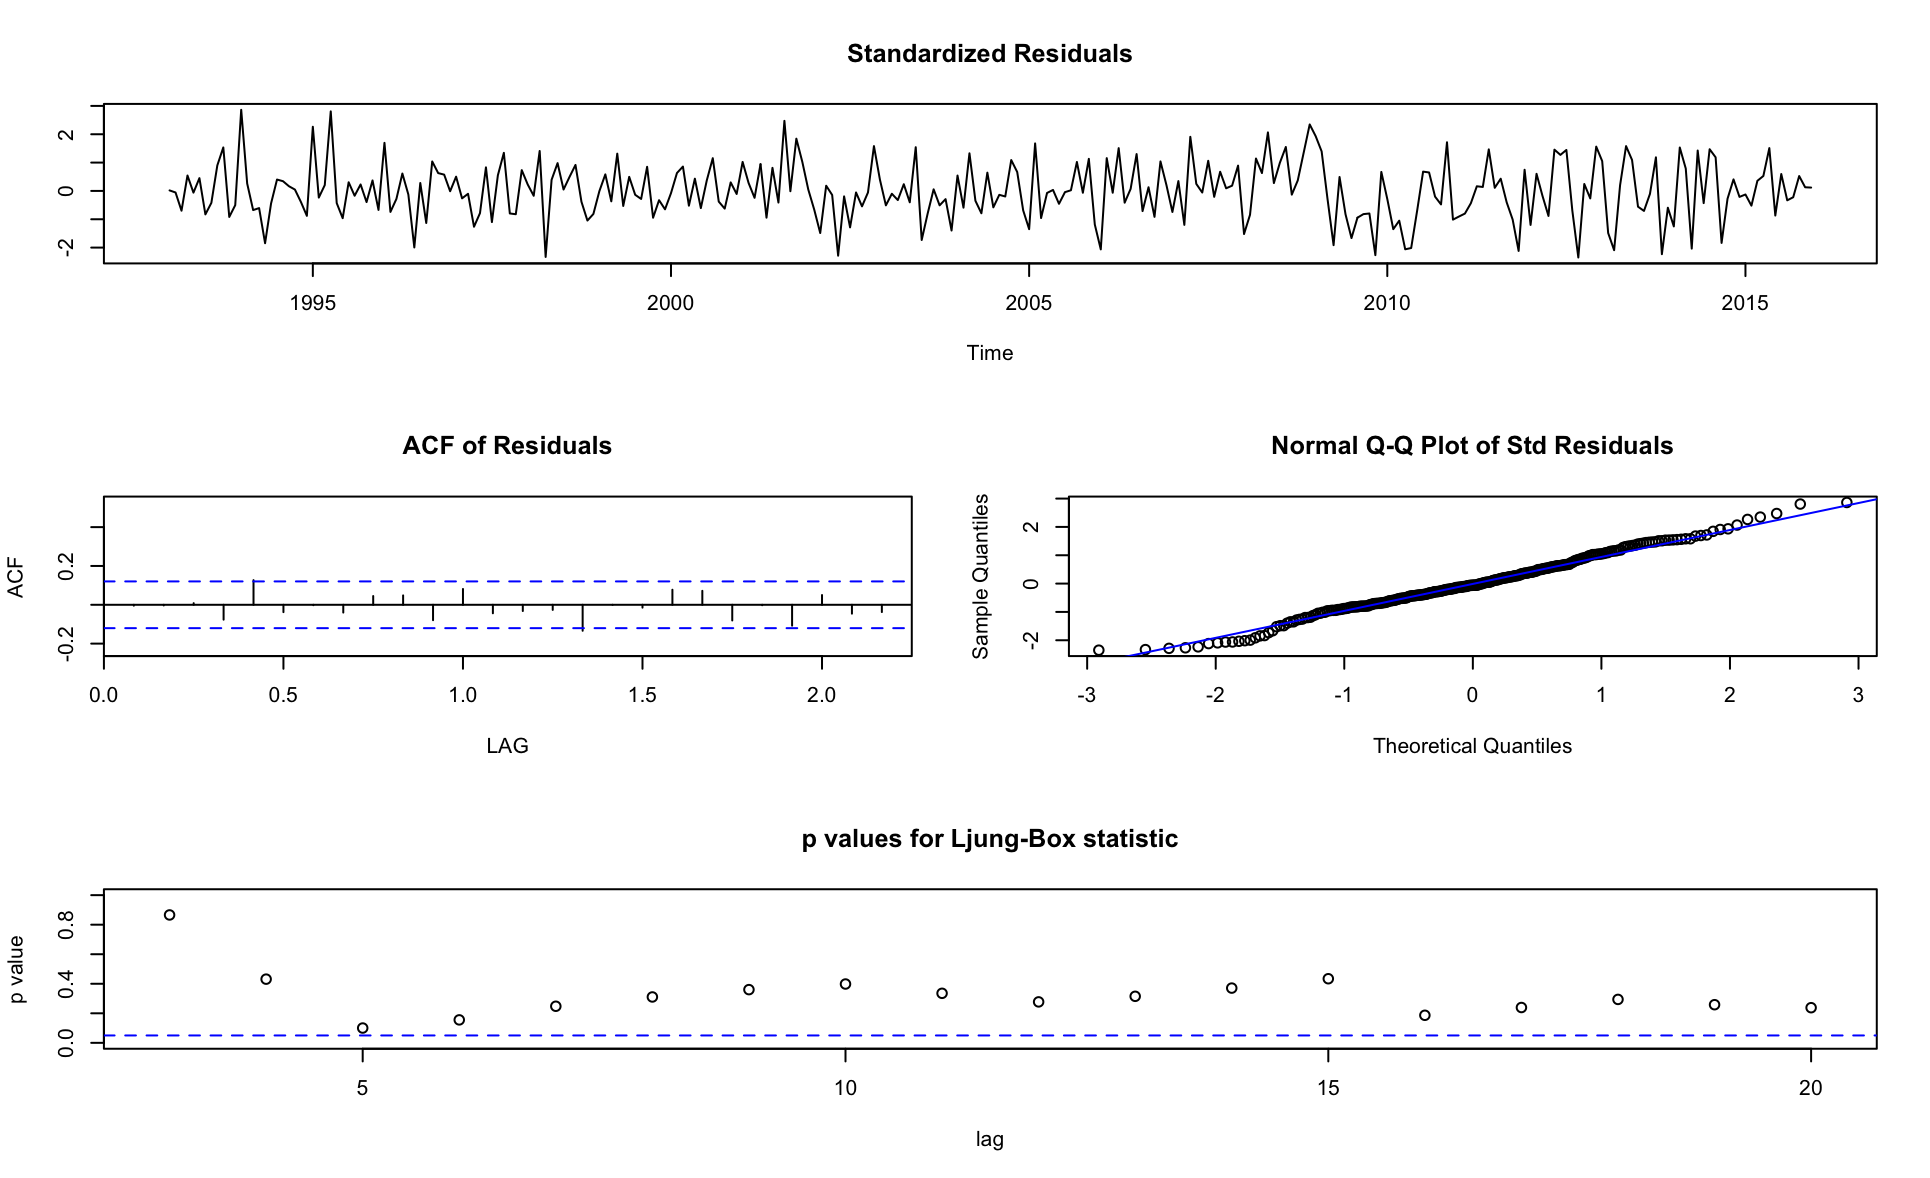
\includegraphics[width=\linewidth]{images/seasonallyadjustedmodel7}
  \end{frame}  
  
  

  %-----------------------------------------------------------------------------------------
  

\end{document}